#import "@local/bootlin:0.1.0": *

#import "@local/bootlin-yocto:0.1.0": *

#import "@local/bootlin-utils:0.1.0": *

#import "../../typst/local/themeBootlin.typ": *

#import "../../typst/local/common.typ": *

#show: bootlin-theme.with( aspect-ratio: "16-9", config-common(handout: "handout" in sys.inputs and sys.inputs.handout == "1", ))

#show raw.where(block: true): set block(fill: luma(240), inset: 1em, radius: 0.5em, width: 100\%)

#show raw.where(block: true): set text(size: 11pt)

#show raw.where(block: false): r => text(fill: color-link)[#r]

#show raw.where(lang: "c", block: true): set block(fill: luma(240), inset: 0.4em, radius: 0.5em, width: 95\%, breakable: true, above: 12pt, below: 12pt)

#show raw.where(lang: "c", block: true): set text(11pt)

#show raw.where(lang: "console", block: true):set block(fill: luma(240), inset: 0.4em, radius: 0.5em, width: 95\%, breakable: true, above: 6pt)

#show raw.where(lang:"console", block: true): set text(12pt)

=== Shopping list: hardware for this course
  
#columns(gutter: 8pt)[
    \begin{itemize}
      \item BeagleBone Black or BeagleBone Black Wireless - Multiple distributors: \\
	    See \url{https://www.beagleboard.org/boards}.
      \item 5V power supply, at least 2A, for the BeagleBone Black, with a 5.5 mm barrel
            jack connector. Needed to drive the LCD cape!\\
	    \url{https://www.olimex.com/Products/Power/SY1005E/}
      \item USB Serial Cable - 3.3 V - Female ends (for serial console): \\
	    \url{https://www.olimex.com/Products/USB-Modules/Interfaces/USB-SERIAL-F}
      \item Beagle Bone Black LCD4.3 cape from 4D systems\\
            \url{https://4dsystems.com.au/products/4dcape-43/}
      \item A standard micro SD card - 1 GB or more
      \item A faster micro SD card - 1 GB or more
    \end{itemize}
     #colbreak()
    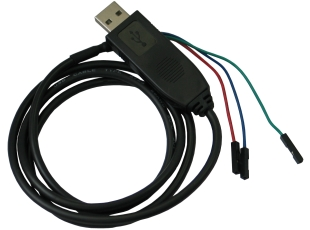
\includegraphics[height=0.20\textheight]{common/usb-serial-cable-female.png} \\
    
\includegraphics[height=0.20\textheight]{common/sd-card.pdf} \\
  \\]

